\documentclass{article}

\usepackage{graphicx}
\usepackage{tikz}
\usepackage{tikzsymbols}
\usetikzlibrary{calc,patterns,shapes.geometric}
\pagestyle{empty}
\usepackage[margin=0pt]{geometry}
\geometry{papersize={14in,12in}}

\def\centerarc[#1](#2)(#3:#4:#5){\draw[#1] ($(#2)+({#5*cos(#3)},{#5*sin(#3)})$) arc (#3:#4:#5);}

\begin{document}
	\begin{figure}
		\centering
		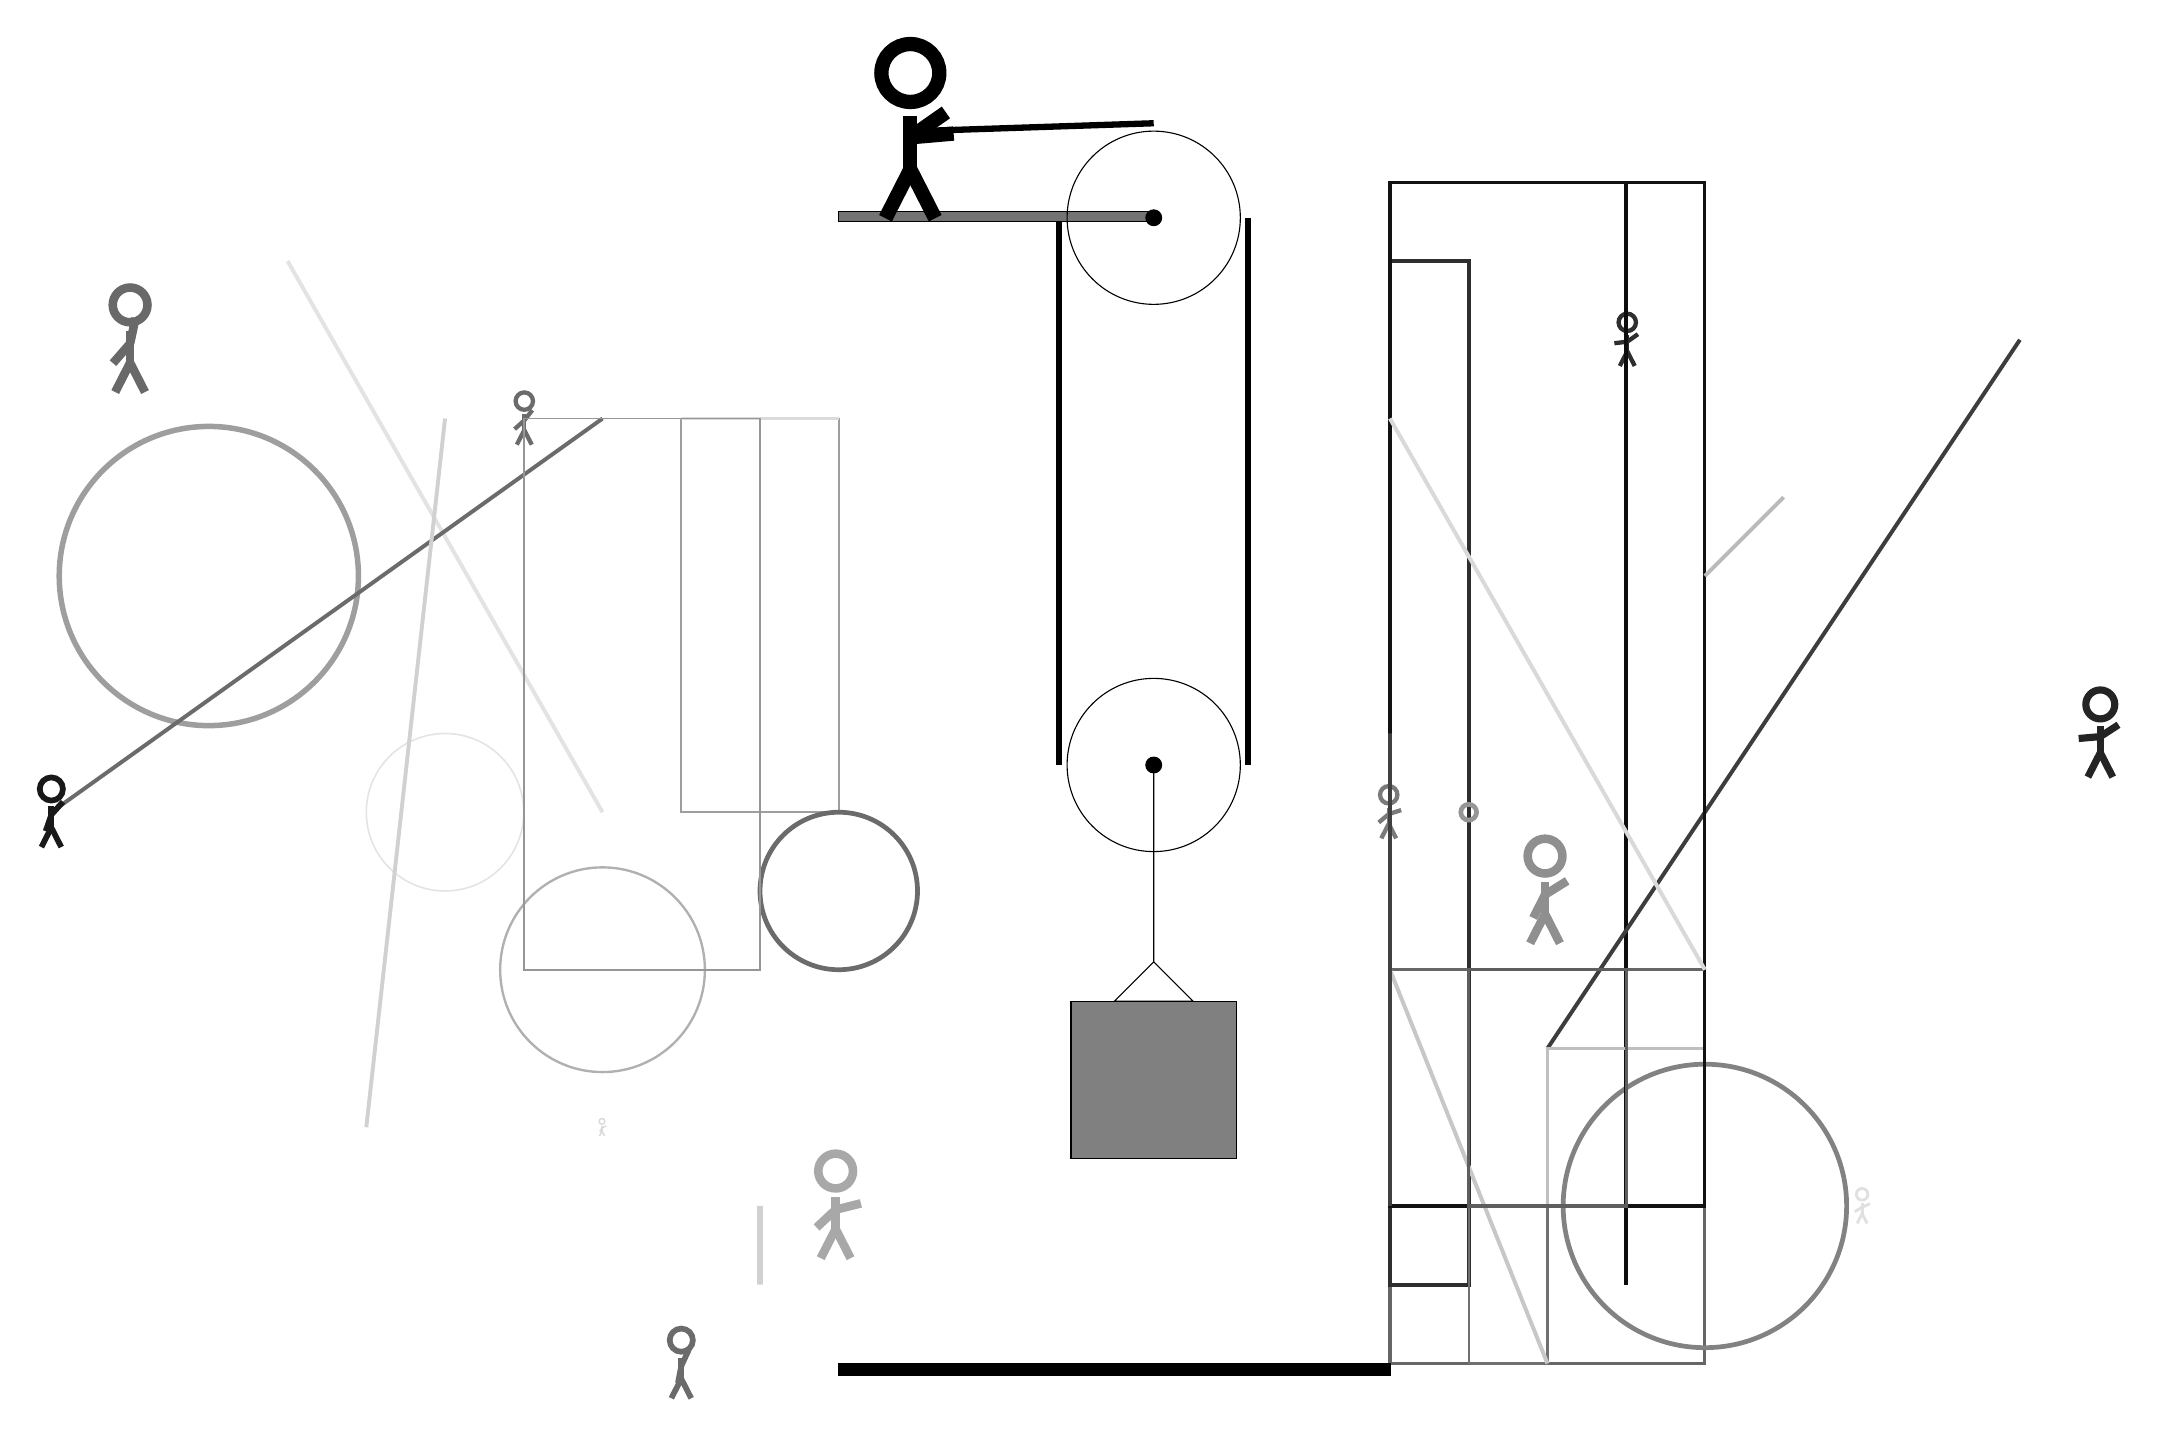
\begin{tikzpicture}
			%%%%% START %%%%%
			
			\draw[fill=black!55] (-2, 11.5) rectangle (2, 11.625);
			
			\draw (2, 4.6) circle (1.1);
			\draw[fill=black] (2, 4.6) circle (0.1);
			
			\draw (2, 11.55) circle (1.1);
			\draw[fill=black] (2, 11.55) circle (0.1);
			
			\draw (2, 4.6) -- (2, 2.1) -- (1.5, 1.6) -- (2.5, 1.6) -- (2, 2.1);
			\draw[fill=black!50] (0.95, 1.6) rectangle (3.05, -0.4);
			
			\draw[line width=0.4mm, color=black!60] (5, 2) rectangle (9, -3);
			
			\node[line width=0.6mm, color=black!59] at (-11, 10) {\Strichmaxerl[6][49][78]};
			\draw[line width=0.5mm, color=black!11](-5, 4) -- (-9, 11);
			\draw[line width=0.5mm, color=black!82] (5, 11) rectangle (6, -2);
			
			\node[line width=0.4mm, color=black!82] at (8, 10) {\Strichmaxerl[3][7][35]};
			\draw[line width=0.2mm, color=black!35] (7, -1) rectangle (7, 1);
			\node[line width=0.6mm, color=black!15] at (-5, 0) {\Strichmaxerl[1][59][25]};
			
			\draw[line width=0.3mm, color=black!56] (6, -1) rectangle (7, -3);
			\draw [line width=0.6mm, color=black!49](9, -1) circle (1.8);
			\draw[line width=0.5mm, color=black!22](7, -3) -- (5, 2);
			
			\draw [line width=0.7mm, color=black!38](-10, 7) circle (1.9);
			\draw[line width=0.5mm, color=black!95](8, -2) -- (8, 12);
			\draw[line width=0.7mm, color=black!18] (-3, -1) rectangle (-3, -2);
			
			\draw[line width=0.5mm, color=black!58](-5, 9) -- (-12, 4);
			\draw [line width=0.2mm, color=black!11](-7, 4) circle (1.0);
			\node[line width=0.2mm, color=black!52] at (5, 4) {\Strichmaxerl[3][40][18]};
			\node[line width=0.5mm, color=black!90] at (-12, 4) {\Strichmaxerl[4][71][48]};
			
			\draw[line width=0.2mm, color=black!38] (-4, 9) rectangle (-2, 4);
			\draw[line width=0.5mm, color=black!76](7, 1) -- (13, 10);
			
			\draw[line width=0.4mm, color=black!25] (7, -1) rectangle (9, 1);
			\draw[line width=0.5mm, color=black!18](-7, 9) -- (-8, 0);
			\draw[line width=0.4mm, color=black!93] (5, 12) rectangle (9, -1);
			\draw[line width=0.3mm, color=black!14] (-2, 9) rectangle (-4, 9);
			\draw[line width=0.5mm, color=black!15](9, 2) -- (5, 9);
			\draw [line width=0.6mm, color=black!58](-2, 3) circle (1.0);
			\node[line width=0.6mm, color=black!58] at (-4, -3) {\Strichmaxerl[4][79][65]};
			\draw [line width=0.6mm, color=black!41](6, 4) circle (0.1);
			\node[line width=0.5mm, color=black!34] at (-2, -1) {\Strichmaxerl[6][43][14]};
			\node[line width=0.3mm, color=black!12] at (11, -1) {\Strichmaxerl[2][31][24]};
			\draw[line width=0.4mm, color=black!63] (6, 2) rectangle (8, -1);
			\node[line width=0.2mm, color=black!58] at (-6, 9) {\Strichmaxerl[3][42][52]};
			
			\draw[line width=0.5mm, color=black!75] (5, -1) rectangle (5, 5);
			\node[line width=0.3mm, color=black!44] at (7, 3) {\Strichmaxerl[6][63][32]};
			\draw [line width=0.3mm, color=black!31](-5, 2) circle (1.3);
			\draw[line width=0.2mm, color=black!41] (-3, 2) rectangle (-6, 9);
			\node[line width=0.5mm, color=black!86] at (14, 5) {\Strichmaxerl[5][5][33]};
			\draw[line width=0.5mm, color=black!27](10, 8) -- (9, 7);
			
			\draw[line width=0.8mm] (0.8, 11.5) -- (0.8, 4.6);
			\centerarc[line width=0.8mm](2, 4.6)(180:360:1.2000000000000002);
			\draw[line width=0.8mm](3.2, 4.6) -- (3.2, 11.55);
			\centerarc[line width=0.8mm](2, 11.55)(0:90:1.2000000000000002);
			\draw[line width=0.8mm](2, 12.75) -- (-1, 12.65);
			
			\node at (-1, 12.65) {\Strichmaxerl[10][-175][35]};
			
			\draw[fill=black] (-2, -3) rectangle (5, -3.15);
			
			%%%%% END %%%%%
		\end{tikzpicture}
	\end{figure}	
\end{document}